\documentclass[sigconf]{acmart}

\usepackage{booktabs} % For formal tables


% Copyright
%\setcopyright{none}
%\setcopyright{acmcopyright}
%\setcopyright{acmlicensed}
\setcopyright{rightsretained}
%\setcopyright{usgov}
%\setcopyright{usgovmixed}
%\setcopyright{cagov}
%\setcopyright{cagovmixed}


% DOI
\acmDOI{10.475/123_4}

% ISBN
\acmISBN{123-4567-24-567/08/06}

%Conference
\acmConference[PDSW-DISCS 2017]{2nd Joint International Workshop on Parallel Data Storage \& Data Intensive Scalable Computing Systems}{November 2017}{Denver, Colorado USA} 
\acmYear{2017}
\copyrightyear{2017}

\acmPrice{15.00}


\begin{document}
\title{Petrel: A Research Data Acceleration Service}

\author{Benjamin Allen, William Allcock, Rachana Ananthakrishnan,\\Ben Blaiszik, Kyle Chard, Ian Foster, and Michael Papka}
\affiliation{%
  \institution{Argonne National Laboratory}
  \streetaddress{9700 S Cass Ave, Lemont, IL 60439, USA}
%  \city{Lemont} 
%  \state{IL} 
%  \postcode{60439}
}
\renewcommand{\shortauthors}{B. Allen et al.}


\begin{abstract}

Data-intensive science requires new data services beyond those provided by conventional
high-performance computing systems.
We established the Petrel data server at Argonne National Laboratory in 2015 to experiment with the utility and operation of such services.
This high-capacity, high-speed data store was configured to enable both interactive Web access
and programmatic access via REST APIs and associated 


Petrel is a data management service operated by the Argonne Leadership Computing Facility (ALCF)
that allows researchers to store large datasets and easily share those data with collaborators. 
%Researchers from the Argonne Leadership Computing Facility (ALCF) and Globus are developing the system collaboratively. 
Petrel leverages ALCF
storage and infrastructure and Globus transfer and sharing services to provide a mechanism for researchers to transfer data into the system, manage data on the filesystem, and share and transfer data to other locations. Authentication and identity to access the system is provided through Globus and users can access Petrel using their campus or institution federated login.
We report here on the design, implementation, applications, and use of this service.
\textbf{The paper is to be submitted to \url{http://www.pdsw.org/index.shtml}. Five pages plus references. Due September 1.}
\end{abstract}

%
% The code below should be generated by the tool at
% http://dl.acm.org/ccs.cfm
% Please copy and paste the code instead of the example below. 
%
\begin{CCSXML}
<ccs2012>
 <concept>
  <concept_id>10010520.10010553.10010562</concept_id>
  <concept_desc>Computer systems organization~Embedded systems</concept_desc>
  <concept_significance>500</concept_significance>
 </concept>
 <concept>
  <concept_id>10010520.10010575.10010755</concept_id>
  <concept_desc>Computer systems organization~Redundancy</concept_desc>
  <concept_significance>300</concept_significance>
 </concept>
 <concept>
  <concept_id>10010520.10010553.10010554</concept_id>
  <concept_desc>Computer systems organization~Robotics</concept_desc>
  <concept_significance>100</concept_significance>
 </concept>
 <concept>
  <concept_id>10003033.10003083.10003095</concept_id>
  <concept_desc>Networks~Network reliability</concept_desc>
  <concept_significance>100</concept_significance>
 </concept>
</ccs2012>  
\end{CCSXML}

\ccsdesc[500]{Computer systems organization~Embedded systems}
\ccsdesc[300]{Computer systems organization~Redundancy}
\ccsdesc{Computer systems organization~Robotics}
\ccsdesc[100]{Networks~Network reliability}


\keywords{TBD, TBD, TBD}


\maketitle



\section{Introduction}

As science becomes increasingly data intensive, 
we see a growing need for discipline-based data services. 
For example, researchers may want to distribute data from a disciplinary repository, 
make data collected at a scientific instrument accessible to remote collaborators,
 allow users to upload datasets for analysis (and retrieve results), 
 or accept data for publication in a public archive. 
 Providing such data acceleration services is a natural way for research computing centers to deliver enhanced value to their stakeholders. But implementing and operating such services can be expensive and cumbersome. 

researchers often need to stage, store, share, and distribute large quantities of data.
In response, we designed and deployed Petrel, 
a data service designed to support scientific  

programmatic access for automation 

Conventional research computing facilities are rarely well suited for such purposes,
being designed to support computational projects rather than data distribution.
for example, a person may need an allocation and account before
they can access a data system.

Argonne National Laboratory is home to thousands of intramural scientists and also
operates a variety of scientific user facilities,
including both experimental apparatus such as the Advanced Photon Source,
with its more than 60 beamlines, and supercomputers, such as those operated
by the Argonne Leadership Computing Facility.
These facilities are used by many thousands of scientists annually, who increasingly
face the need 
These facilities and other activities at the lab increasingly involve large 
quantities of data, 
which proved to be surprisingly difficult to manipulate due to the lack of suitable storate facilities 



Petrel represents one sort of expansion of what is traditionally thought of as the role of high-performance computing facilities~\cite{UrPa16}. 
This is in addition to providing a large supercomputers for running traditional simulations, facilities need to evolve to become a highly usable service facility, deeply integrated into science projects and serving as a hub for science communities. 
Petrel introduces a new service that integrates with user environments and workflow to improve the usability and utilization of HPC centers. 
It provides a configurable solution to the sharing of data with colleagues and the community, 
while at the  same time keeping the large datasets close to large computational resources.



\begin{verbatim}
32 Nodes with 1.7 PB usable storage
GPFS and Globus
100TB allocation per project
Transfer and sharing data with collaborators
Federated login
Self-managed by PIs
\end{verbatim}

MRDP~\cite{BMRDP}.

The Materials Data Facility (MDF)~\cite{MDF2016} ...

DEBD~\cite{foster2015networking}.


\section{The Petrel System}

\subsection{Hardware}

Petrel comprises a single IBM Elastic Storage Server (ESS) GL6 plus eight data transfer nodes (DTNs)~\cite{dart2014science} for external access.

An ESS GL6 is configured with two IBM S822L Power8 based servers as IBM General Parallel File System (GPFS)~\cite{schmuck2002gpfs} Network Shared Disk (NSD) servers, and one IBM S812L as a management and provisioning server. 
Each NSD server is connected with 4$\times$FDR10 connections to the same fabric as the DTNs. 
Petrel includes six disk trays with a total of 348 6TB SAS HDDs. 
Configured with 8+2 parity and 3 drives worth of hot spare space, Petrel provided a usable capacity of 1.7P, and was benchmarked via IOR at Max Write: 16,563.06 MiB/sec (17,367.62 MB/sec), Max Read:  23,110.68 MiB/sec (24,233.31 MB/sec).

Each of the eight Petrel DTNs has a single Mellanox ConnectX-4 40GbE NIC, a single Mellanox Connect-IB HBA (running at QDR), 64GB RAM ($\sim$42GB dedicated to GPFS), and a single socket Intel E5-1660 v3 8c @ 3.00GHz CPU. 
Both Mellanox cards sit on PCIe 3.0 x16 buses.

The eight Petrel DTNs are connected to two core Mellanox SX1710 36-port 40GbE switches
maintained within Argonne's Joint Laboratory for Systems Evaluation (JLSE).
%JLSE has two core Mellanox SX1710 36-port 40GbE switches. 
The Petrel DTNs are split across the two switches, each connected with 1$\times$40GbE. 
%The split is along even and odd numbered DTNs. 
Each of the two 40GbE core switches has a 2$\times$40GbE link aggregation group to the ALCF core router, which in turn has a 100GbE connection to the core router for the data center within
which ALCF is located,
%SDN240. 
%At this point we are sharing available bandwidth with ALCF. 
%SDN240 in turns 
which in turn connects at 100GbE to one of the ANL border routers.
Thus, as Petrel traffic reaches beyond JSLE to ALCF, the data center, and the border,
it shares bandwidth with an increasing range of other activities.
%At this point we share available bandwidth with all of the 240 datacenter, 
%and at the border we share with the rest of the lab to ESNet.

\subsection{Software}

GPFS 

Globus




\section{Example User Workflows}


Beamline scientists from Argonne's Advanced Photon Source (APS) use Petrel as a resource for their data management.

The scientists request a project allocation on Petrel. 
Upon approval, they have access to 100TB. 
They also have the right to add other users, to whom they can grant rights to manage, read, and/or write the space.

Once data is generated at APS, scientists transfer it to the project space on Petrel. 
They can then set up permissions to enable remote collaborators to access all or a subset of the data. 
Importantly, remote collaborators do not need Argonne accounts to access the data.

Petrel users can easily stage all or some of their data to a compute resource for analysis, and then move results back to Petrel.



\section{Use Cases}

\subsection{Tomography}

A microtomography research team at Argonne's Advanced Photon Source (APS) collects 20-80TB/month of raw data, and expects to scale to about 100-200TB/month in the near future. Microtomography can be carried out at a variety of energies suitable for 3D characterization of materials relevant to materials science, geoscience, energy storage, and biology. High-speed imaging allows for ultra-short exposure times, allowing for detailed study of transient material phenomena. Researchers in this group get an allocation at the beamline for a duration of a few days, and gather data that needs to be further processed and analyzed. Subsets of the raw data need to be moved to a diverse set of analysis and storage facilities for processing and long-term preservation. Users can leverage Petrel to help meet these requirements. APS beamline users would also like to use Petrel to track their study metadata and provenance, and share raw and analyzed data with collaborators (some working remotely).

Things that mention Petrel: Tekin paper~\cite{bicer2016optimization}. Skluma~\cite{beckman2017skluma}.

\subsection{Materials Science}

A group of scientists from Argonne's Materials Science Division (MSD) gather experimental data from APS beamlines with raw data volumes ranging from 60--100 TB/month with data volumes expected to double by 2016. These scientists require a flexible environment to implement end-to-end experiment-time data analysis workflows to automate their analyses and leverage distributed computing resources. This functionality allows the researchers to compare their experimental data to simulation results drawn from high-performance computing resources to rapidly provide actionable feedback and data visualization. These scientists can leverage Petrel to help meet these requirements.

Through Petrel and Globus functionality, we provide intuitive interfaces for these researchers to share, bundle, and publish their datasets. After data is gathered, the scientists often want to share subsets of raw data, derived datasets, and analysis results with collaborators, track metadata associated with the data, and track data provenance. Eventually, these scientists may want to make their datasets publicly and persistently available via publication functionality, fully bundled with the associated metadata and associated with a persistent identifier to aide search, discovery, and data citability.

\section{Usage Data}

Another fun fact of this system, since we put it into production we have only had a single hard drive fail, and that was just a few weeks ago. Since it was installed we have only had one additional drive fail, which was during early burn-in.

\begin{figure}
\centering
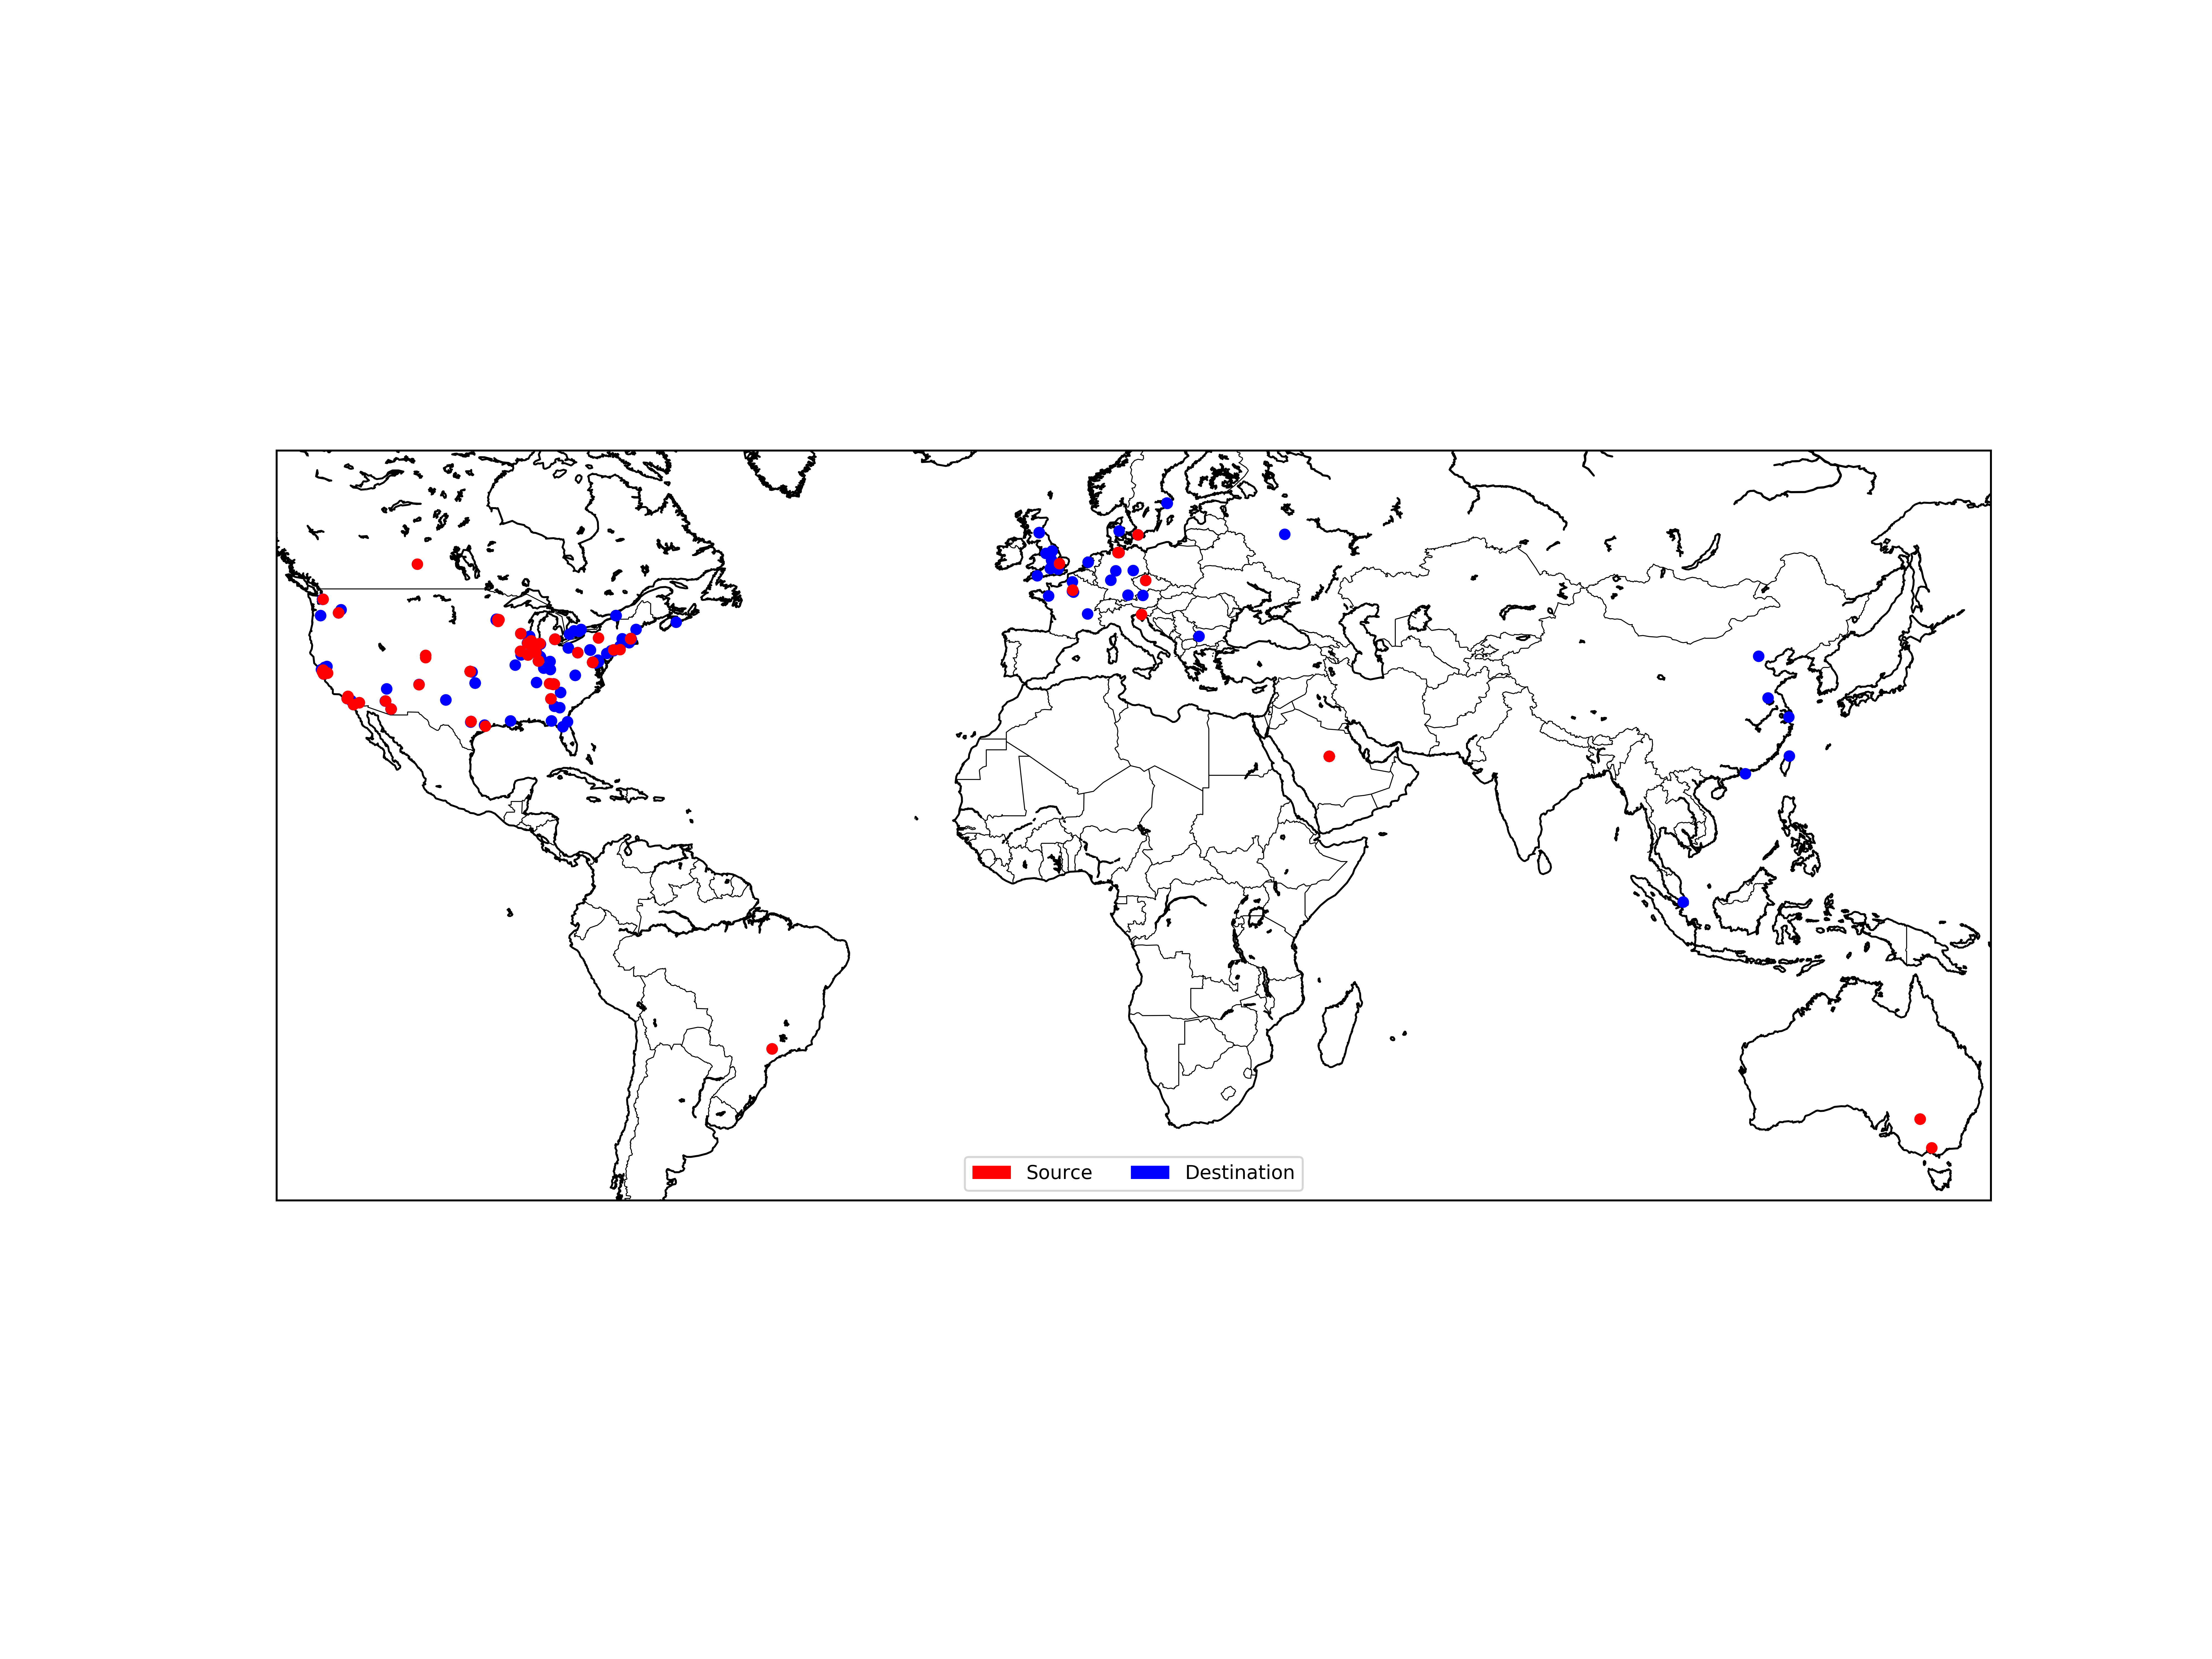
\includegraphics[trim=2in 3.3in 1.4in 3in,clip,width=\columnwidth]{Figures/petrel-src-dst-map2.png}

\vspace{-1ex}

\caption{Petrel source and destination endpoints for which geolocation
data are available.\label{fig:usage1}}
\end{figure}


\begin{figure}
\centering
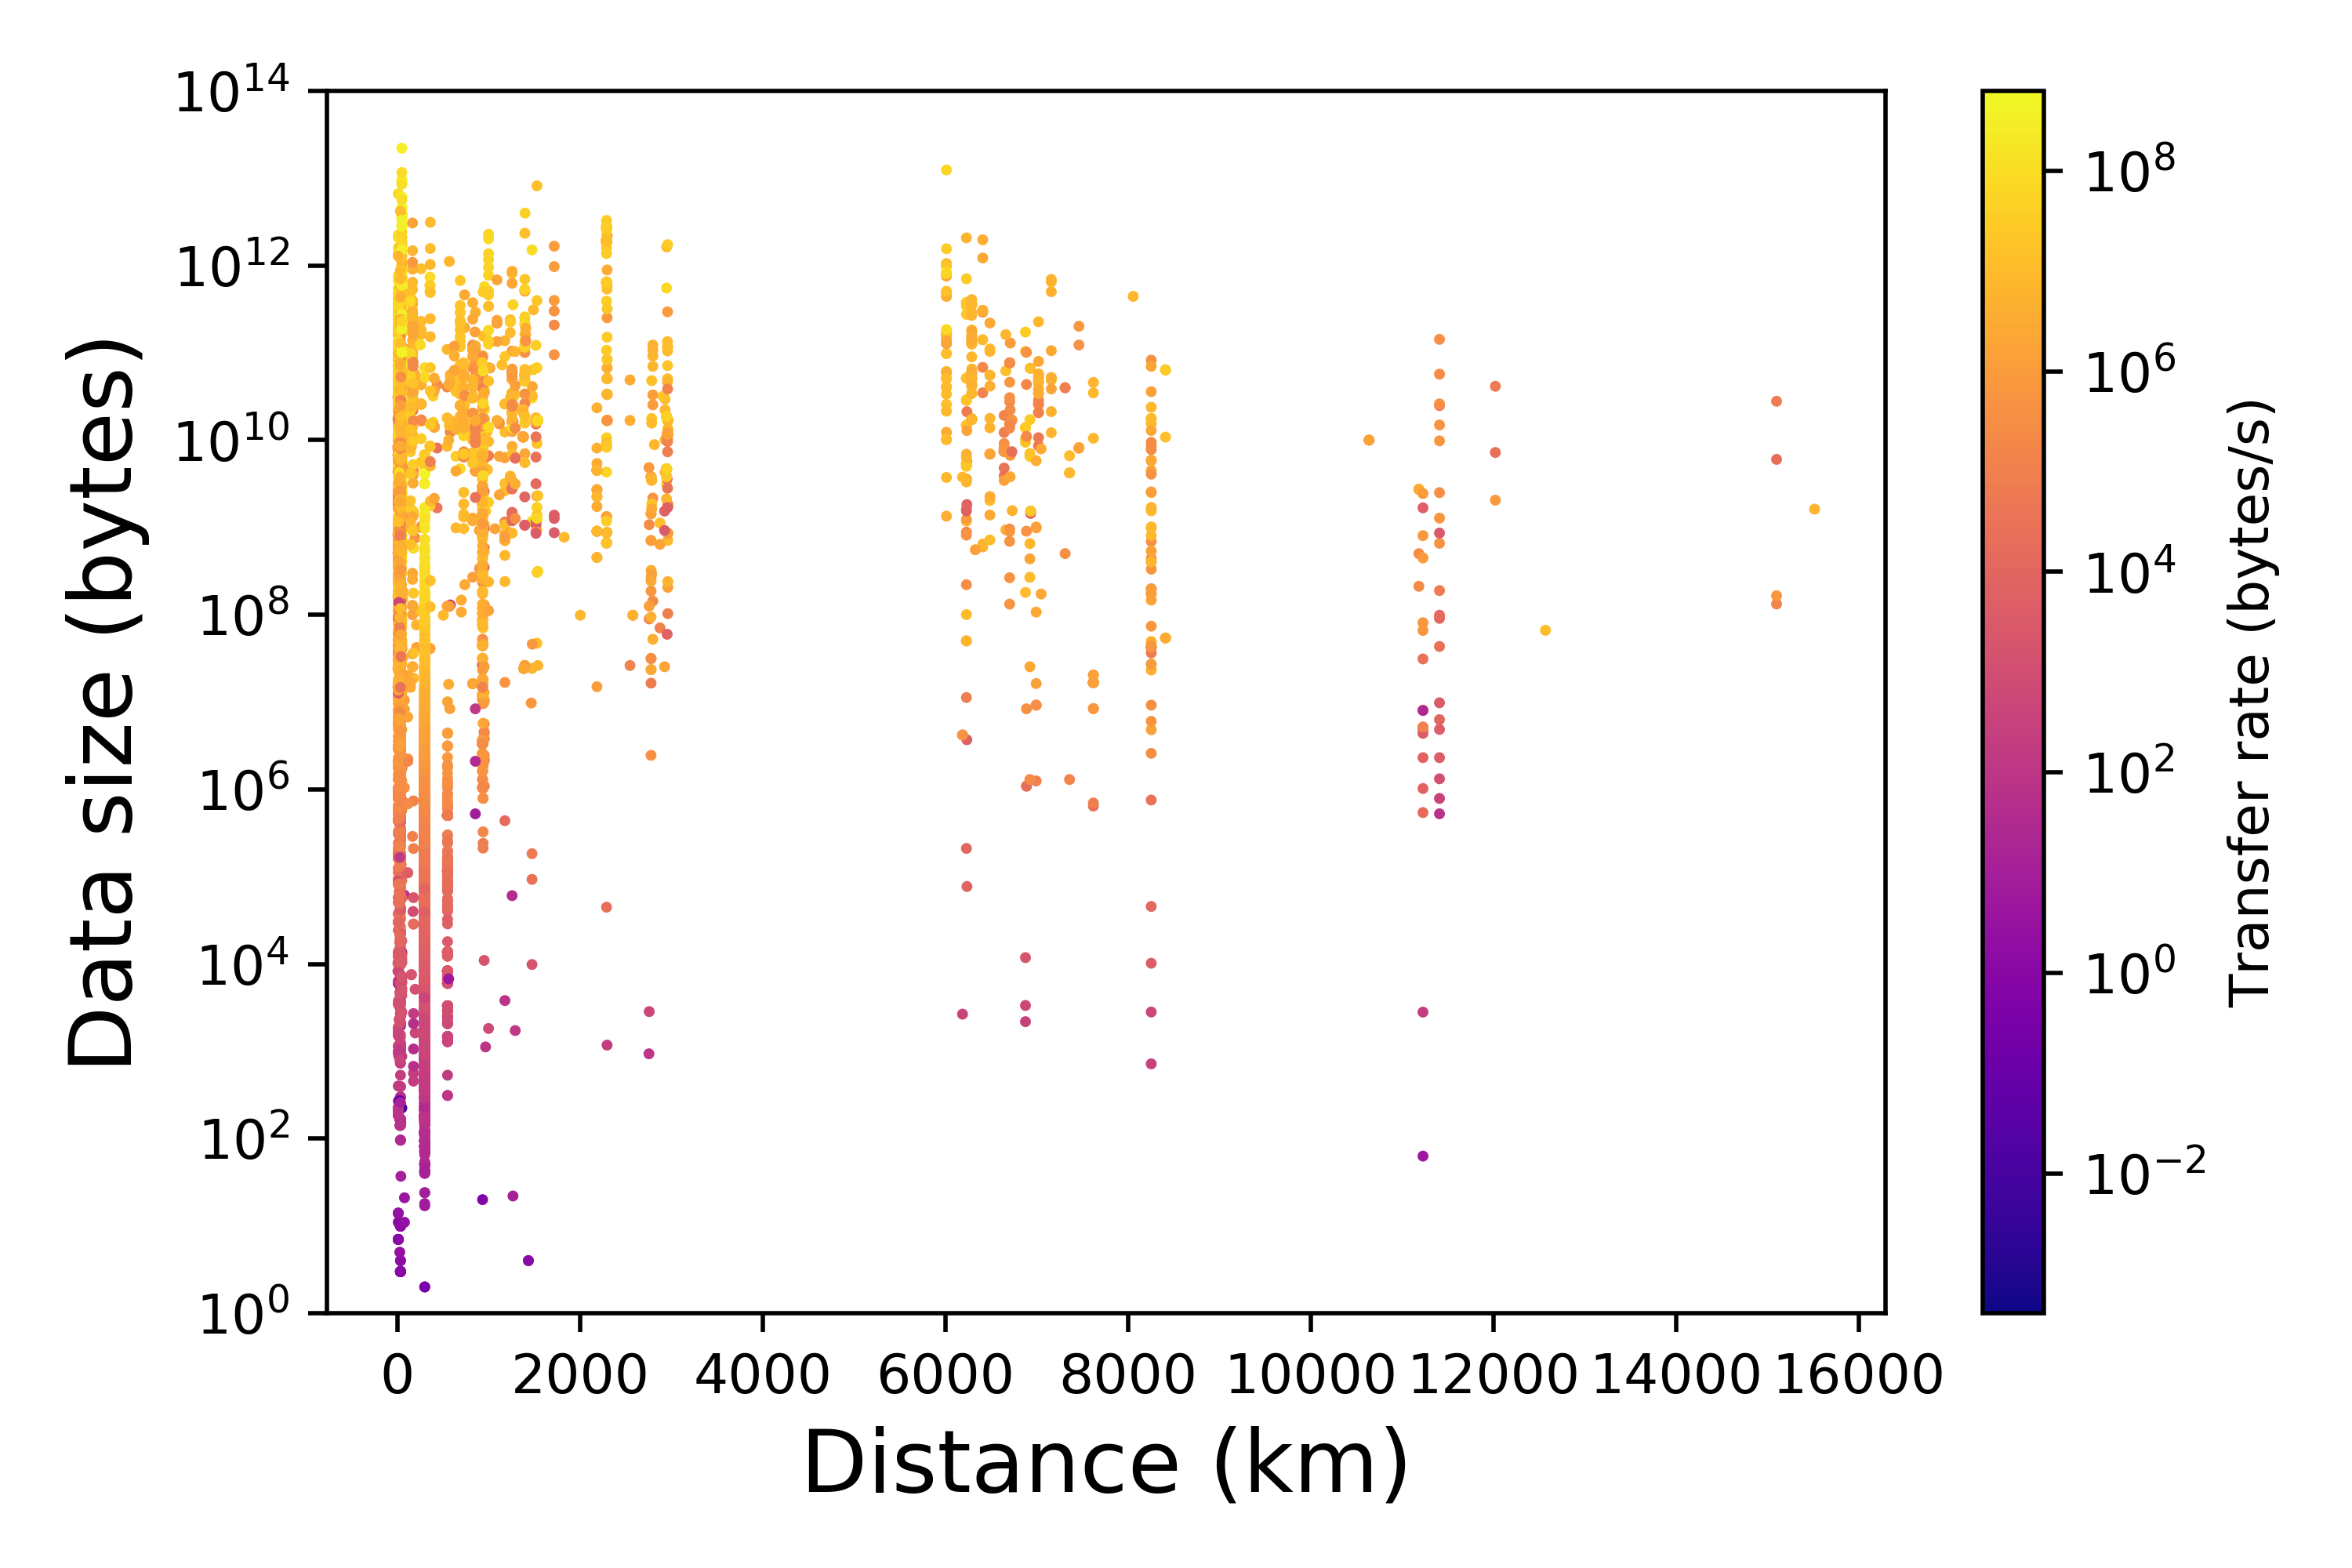
\includegraphics[trim=0.1in 0.1in 0.1in 0.1in,clip,width=\columnwidth]{Figures/size-distance-speed.png}

\vspace{-2ex}

\caption{Each point represents a single transfer,
and gives transfer size vs.\ great circle distance between Petrel and remote source or destination, 
with transfer rate color coded.\label{fig:usage2}}
\end{figure}



\section{Related Work}

Distributed file system ... e.g., AFS 

The Data Capacitor~\cite{simms2007empowering}

wide area file system: Andrew File System~\cite{howard1988scale}, Lustre on TeraGrid~\cite{simms2007wide}

Logistical networking~\cite{beck2000logistical} 




\section{Conclusions}


Today Petrel allows the easy sharing of data with colleagues and the community.
In the future our plan is to enhance Petrel to be able to support the analysis of the data by the same sharing group:
starting with defined analysis infrastructure and over time moving to more generic analysis infrastructure.

\section*{Acknowledgments}
The Argonne Leadership Computing Facility is a DOE Office of Science User Facility supported under contract DE-AC02-06CH11357.


\bibliographystyle{ACM-Reference-Format}
\bibliography{petrel} 

\end{document}
